Money is a social construct, like trust. Both are very important and ephemeral things, and are being tested in a global digital world.  We are a long way from the village structures in which we evolved. We are now expected to casually adapt to the efficiencies promised by teams working in global mixed reality. This chaotic and intangible mix of value, trust, and socialisation is not well understood.\par
We wanted to explore exciting new developments in the transmission of value, and trust, in metaverses. The problem is that each of these topics alone are enormously complex, and the intersections seem to be more so. We have been researching the current state-of-the-art, and the emerging consensus narrative, to try to figure out how the collision of these technologies might serve Pathway XR virtual production studio, and the broader creative communities. \par
We started out with security best practices in mind. How can we enable creative collaboration on a global stage, without their cybersecurity costs spiralling? \par
Fortunately, we discovered a wealth of carefully crafted open source tools which can support this exploration. We have tried to assemble them cogently, to deliver a kit for experimentation, and we have applied our own security knowledge on top of an already top class set of tools. It’s certainly not production ready, but it's good enough to commit small amounts of money into, for experimentation purposes.\par
Whilst researching, it seemed that every door we opened was full of interesting and useful treats. What was supposed to be a short technical paper quickly became a 200-page book, and a deployable virtual machine stack, with a dozen different open source components in it. \par
To that end, this book supports the virtual machine and software stack, which supports anyone who thinks this material might be useful. Below is a précis of the chapters of the book, which will hopefully give an insight into what ``this stuff'' is. The reader can decide to download the book and the system ``How To'' guide. All of it is open source, all of it can be contributed to on GitHub, all of it will be developed forward, and none of it is really finished yet.\par
Chapter 1 is an introduction to the book which is about value transmission, with distributed trust, in global social mixed reality systems. \par
Next is a summary of Web3, as it stands right now. Web3 is a complex term that is cropping up far more in the technical press, so we wanted explain what it might mean. Honestly, it’s still pretty confusing. There are a bunch of legacy explanations which are Web3.0 (note the `0' there), but these are withering on the vine. Then there’s the new VC funded, super hyped, and potentially useless Web3 incarnations, which again cover a slew of intersecting technologies. Note they dropped the zero to reboot the brand! This doesn’t mean there’s nothing to see here. The astonishing amount of \href{https://mirror.xyz/tr3butor.eth/AlZPMq_syymAoi8M1VVb2xES9Twj1OeetJbEE7EWhiw}{money and developer talent}, and the clear market hunger for things like NFTs (non-fungible tokens) suggest that there’s a future for Web3.\par
In the next chapter we took a look at blockchain, which is very intersectional with Web3. Even on its own this is a very complex emergent set of disciplines. \par
The blockchain chapter was especially interesting to research. It turns out there’s a \textit{lot} of ways to get this technology wrong, and this was covered in the first edition of the book. The edition you are reading is more focused and dropped everything else in favour of Bitcoin. Earlier versions are available in the GitHub. \par
Even Bitcoin isn’t just Bitcoin anymore. It’s a swarm of open source tools which can (in theory) accomplish a great many things. These newer, ancillary elements to Bitcoin, are emergent right now. Some of them won’t be around until next year and it’s questionable whether they will even work out. With that said there’s already enough here for us to cherry pick some useful components and start to map those forward into our metaverse proposal.\par
In looking around at the available options, it seems possible that the features which are important to Web3, can also (potentially) arise from the Bitcoin technology that we think most secure.\par
The next chapter is about Money. In expanding our research on Bitcoin, we found that it’s impossible to think about the tech without opening up a whole line of questions about money itself. This is fine because we set out to look at global value transfer for business. It’s not a trivial subject though, and this section tries to overview why value and Bitcoin are so enmeshed, then what other options there might be in the end (because Bitcoin has kicked off a whole slew of global adoption outside of itself).\par
The distributed identity management, and trust chapter follows. Identity management is crucial to metaverse applications which have a value transaction layer. It’s not an easy section to write about, because there’s a lot of research, it’s not our field, and finding the value to SMEs has actually been very difficult. It's by no means clear that blockchain is the right tool for this component, and newer cryptographic products are emerging. This section is likely to be overhauled a few times in the coming months as we settle on technologies that we believe are simple and secure enough.\par
In chapter 7 we take another look at NFTs. It’s impossible to ignore this stuff now that Meta has integrated them into \href{https://twitter.com/MetaNewsroom/status/1564281969134927872}{both Instagram and Facebook in 100 countries}. It’s fundamentally a bit broken, but there are probably use cases, and the money and development attention it’s getting are incredible.\par
We’re actually pretty excited about future versions of this technology, based around Bitcoin, because that allows us to keep just one value stack for our virtual production creative. Keep it simple. We’ve mapped that forward into the open source tools that we recommend. \par
Chapter 8 is a big one for us as it’s our research area prior to opening up the Bitcoin box(es). Metaverse, or at least one of the current definitions of metaverse, is just social interaction in mixed reality (VR/AR/XR). We’ve been studying that for decades, so this section is more academic and tried to boil down what we think is most important to map forward into the server stack. The choices we made here guided us toward the selection of free and open source metaverse software, which we selected from a bunch that we reviewed. We also obviously will have to describe Unreal for virtual production, but this isn't done yet.\par
We also take a look at the other definitions of metaverses which are doing the rounds on the web, try to unpick which is which, and what they are for, then we attempt to weave back together the best of both. This ends up looking a bit like the Venn in Figure \ref{fig:landscapevenn}, where we have transmission of provable identity, non-fungible tokens bearing value or data, distributed files, actual money (including micropayments) and a social layer based on our best knowledge about mixed reality. Figure \ref{fig:landscapevenn} is really the culmination of the research and can be considered a teaser.\par
\begin{figure*}[ht]\centering % Using \begin{figure*} makes the figure take up the entire width of the page
	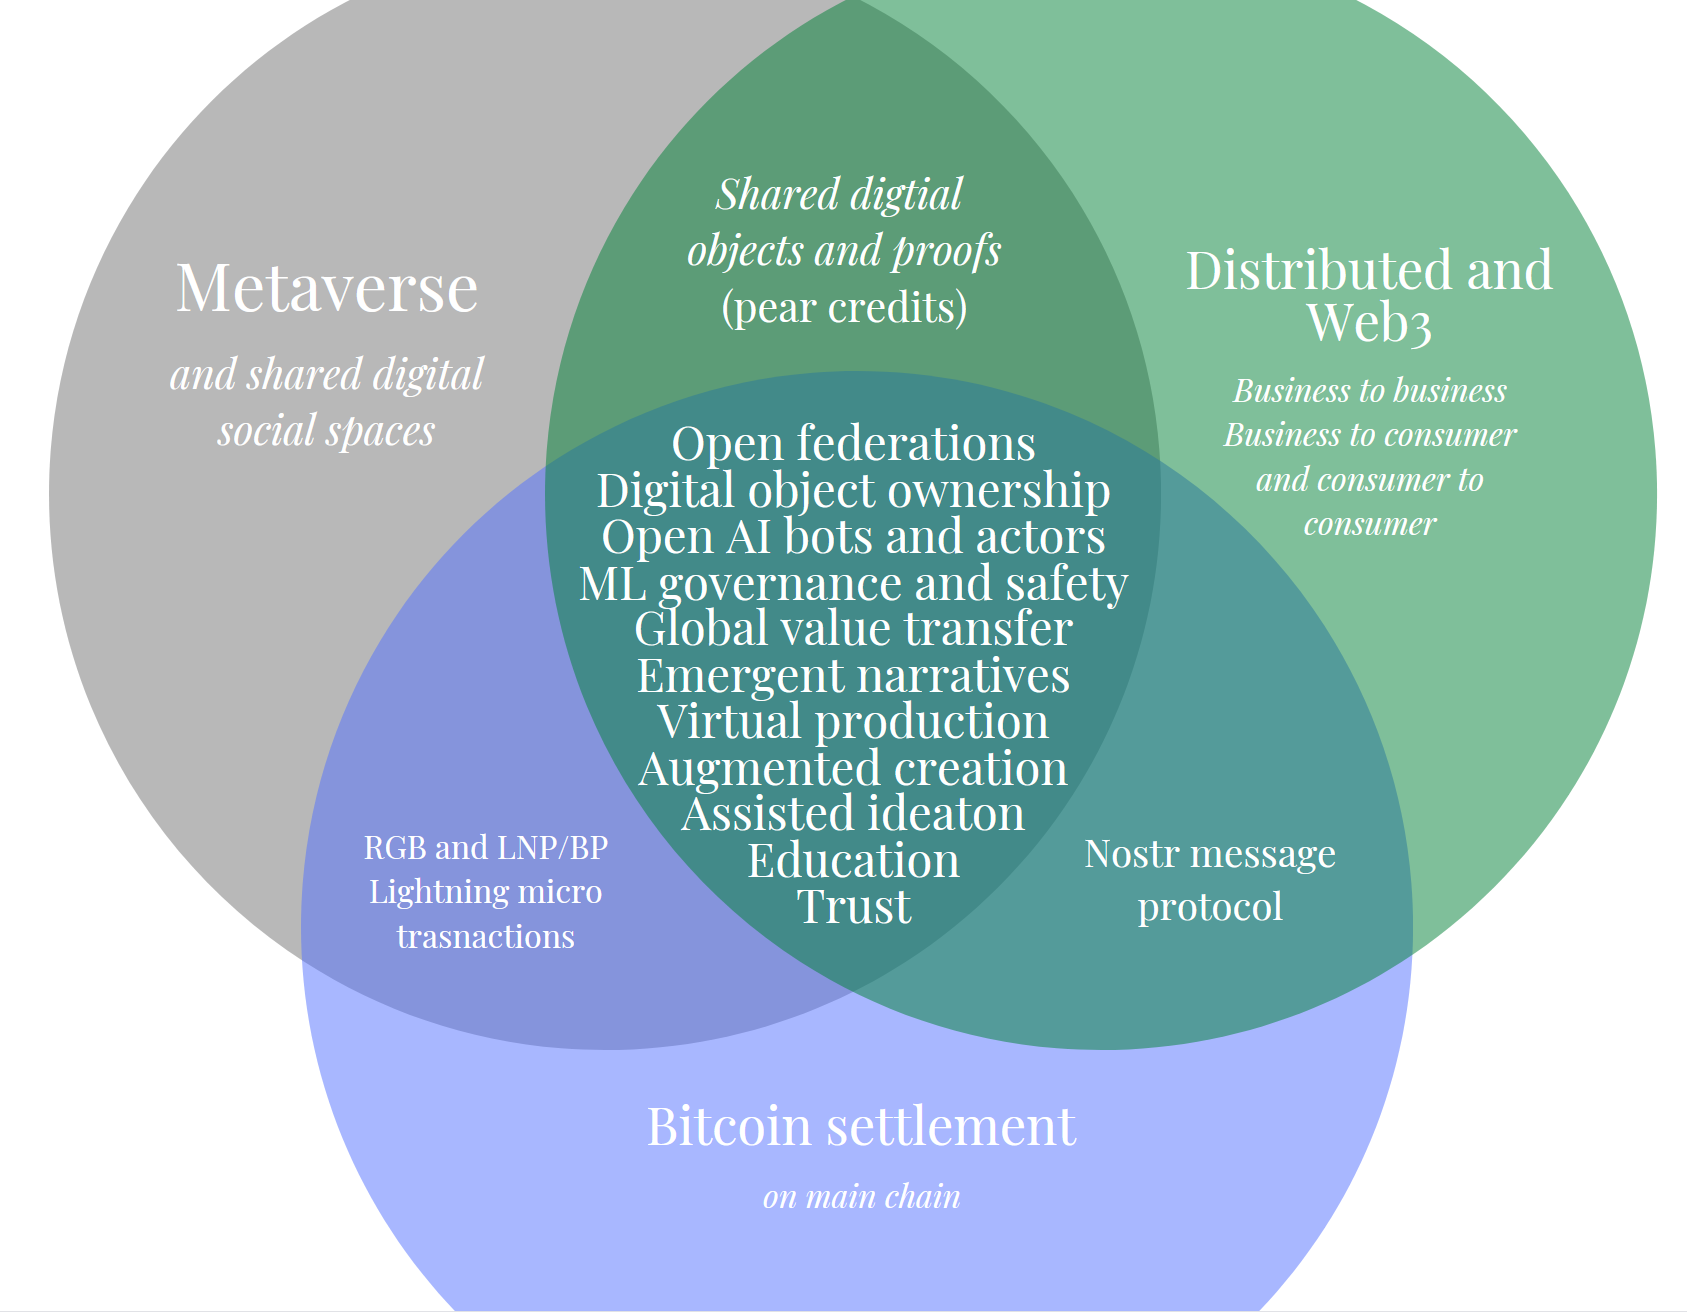
\includegraphics[width=\linewidth]{landscapevenn}
	\caption{Web 3, Metaverse, and Bitcoin are inter-sectional technologies.}
	\label{fig:landscapevenn}
\end{figure*}
It's exceptionally fortunate timing for this book that the UK government has signalled enthusiasm for so called `stablecoins' at the same time that the Bitcoin network is being upgraded to transmit these GBP equivalent tokens around. This gives us a very good idea what it is we can build into our application stack.\par 
Past this stage in the book we get into the murky and half developed tail end, where we’re interfacing with our design choices, and the stack which can be deployed into the cloud.


